\documentclass[11pt]{amsart}

%%%%%%%%%%%%%%%%%%%%%%%%%%%%%%%%%%%%%%%%%%%%%%%%%%%%%%%%%%%%%%%%%%%%%%%%%%%%
%% Standard AMS packages
\usepackage{amsthm,amsmath,amssymb,amscd,thmtools}
\usepackage[pdftex, plainpages=false]{hyperref}   %% Hyper-references - To be use with PDF-TEX
\usepackage{amsfonts, mathrsfs}
\usepackage{lineno}
\usepackage{commands}
\usepackage{tikz,tikz-cd}
\usetikzlibrary{calc}


\begin{document}

\title{Homework 1}


\maketitle


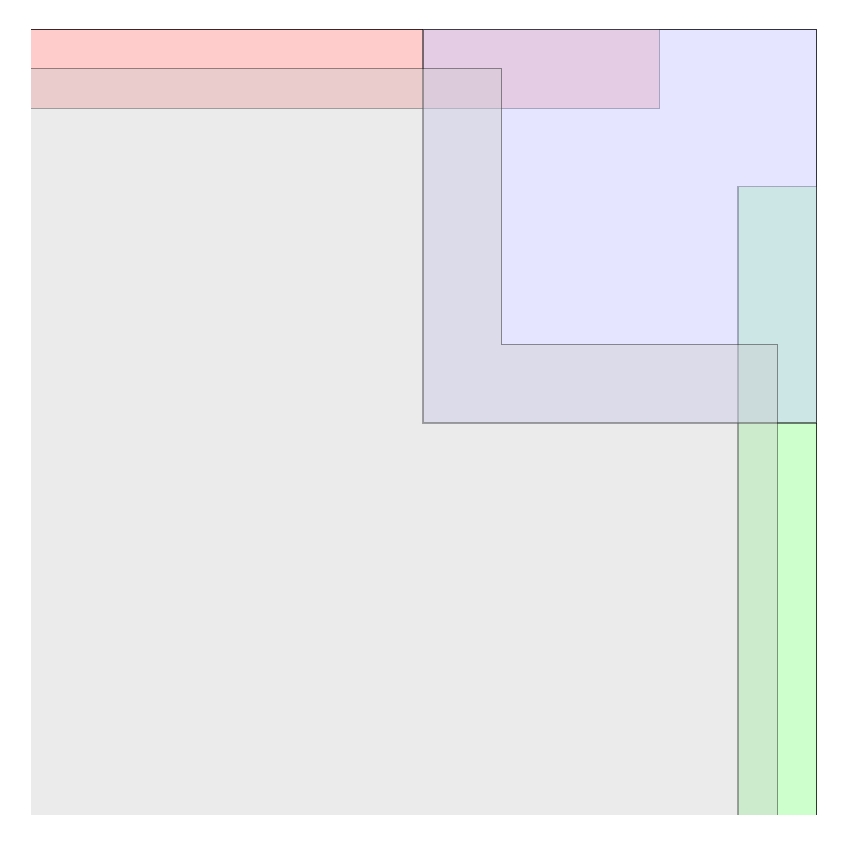
\begin{tikzpicture}
\draw (0,10) -- (10,10) -- (10, 0);
\filldraw[fill=red!40, opacity=0.5](0,9) rectangle (8,10);
\filldraw[fill=green!40, opacity=0.5](9,0) rectangle (10,8);
\filldraw[fill = blue!20, opacity = 0.5](5,5) rectangle (10,10);
\filldraw[fill = black!20, opacity = 0.4] (0,9.5) -- (6,9.5) -- (6,6) -- (9.5,6) -- (9.5, 0) -- (0,0) -- (0, 9.5);
\draw[white, very thick] (10, 0) -- (0,0) -- (0,10);
\end{tikzpicture}



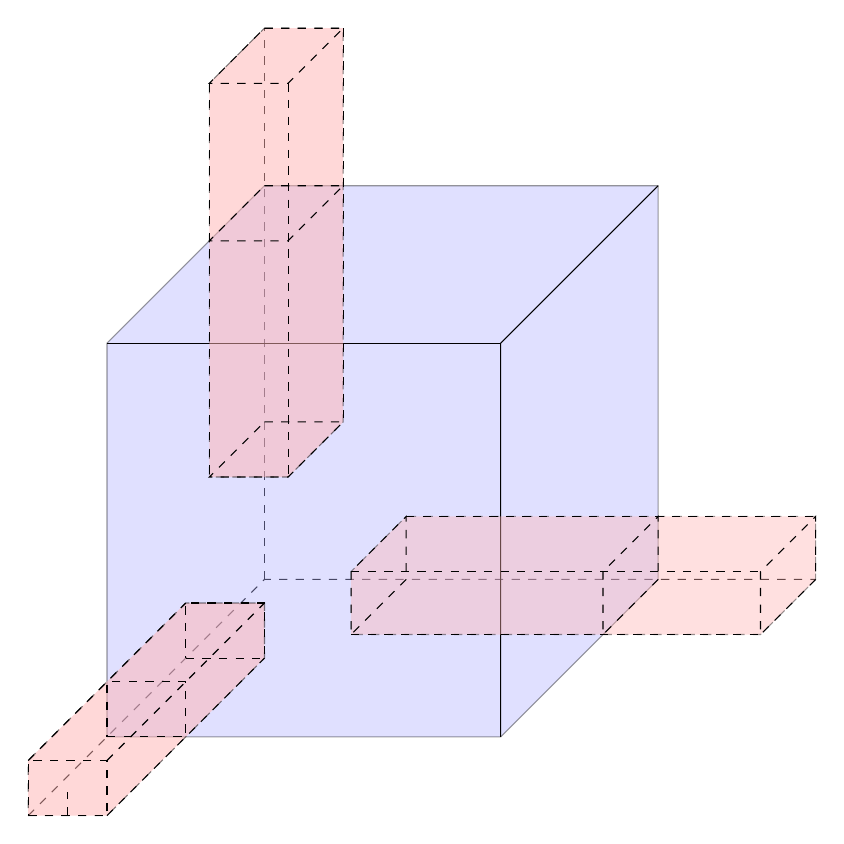
\begin{tikzpicture}
% the coordiante and the large box
\draw[dashed] (0,0) -- (3,3) -- (10,3);
\draw[dashed] (3,3) -- (3,10);
\filldraw[fill = blue!30, opacity = 0.4] (1,1) -- (6,1) -- (8,3) -- (8,8) -- (3,8) --(1,6) -- (1,1);
\draw (6,1) -- (6,6) -- (8,8);
\draw (6,6) -- (1,6);

% constants
\coordinate (p4) at (1.7, 1.7);
\coordinate (p5) at (3,3);
% % small box
% \coordinate (bdy) at (2.7,0);
% \coordinate (bdz) at (0, 3.3);
% \coordinate (bdx) at (2,3);

% \filldraw[dashed, fill = blue!30, opacity = 0.7] (p4) -- ($(p4) + (bdy)$) -- ($(p5) + (bdy)$) -- ($(p5) + (bdy) + (bdz)$) -- ($(p5) + (bdz)$) -- ($(p4) + (bdz)$)--  (p4);

% \draw[dashed] (p4) -- ($(p4) + (bdy)$) -- ($(p4) + (bdy) + (bdz)$) -- ($(p4) + (bdz)$) -- (p4);
% \draw[dashed] (p5) -- ($(p5) + (bdy)$) -- ($(p5) + (bdy) + (bdz)$) -- ($(p5) + (bdz)$) -- (p5);

% \draw[dashed] ($(p4) + (bdy) + (bdz)$) -- ($(p5) + (bdy) + (bdz)$);
% \draw[dashed] ($(p4) + (bdz)$) -- ($(p5) + (bdz)$);
% \draw[dashed] ($(p4) + (bdy)$) --($(p5) + (bdy)$);



% lower left
\coordinate (p1) at (0,0);
\coordinate (p2) at (1,1);
\coordinate (p3) at (2,2);


\coordinate (dx) at (1,1);
\coordinate (dy) at (1,0);
\coordinate (dz) at (0, 0.7);



% \filldraw[dashed, fill = red!40, opacity = 0.5]  (p2) -- ($(p2) + (dy)$) -- ($(p3) + (dy)$) -- ($(p3) + (dy) + (dz)$) -- ($(p3) + (dz)$) -- ($(p2) + (dz)$) -- (p2);


\filldraw[dashed, fill = red!30, opacity = 0.5] (p1) -- ($(p1) + (dy)$) -- ($(p3) + (dy)$) -- ($(p3) + (dy) + (dz)$) -- ($(p3) + (dz)$) -- ($(p1) + (dz)$) -- (p1);

\draw[dashed]         (p1) --  ($(p1) + (dy)$) -- ($(p1) + (dy) + (dz)$) -- ($(p1) + (dz)$) -- (p1);
\draw[dashed] (p2) --  ($(p2) + (dy)$) -- ($(p2) + (dy) + (dz)$) -- ($(p2) + (dz)$) -- (p2);
\draw[dashed] (p3) --  ($(p3) + (dy)$) -- ($(p3) + (dy) + (dz)$) -- ($(p3) + (dz)$) -- (p3);
%\draw[dashed] (p4) --  ($(p4) + (dy)$) -- ($(p4) + (dy) + (dz)$) -- ($(p4) + (dz)$) -- (p4);


\draw[dashed] ($(p1) + (dy)$) -- ($(p2) + (dy)$) -- ($(p3) + (dy)$);
\draw[dashed] ($(p1) + (dy) + (dz)$) -- ($(p2) + (dy) + (dz)$) -- ($(p3) + (dy) + (dz)$);
\draw[dashed] ($(p1) + (dz)$) -- ($(p2) + (dz)$) -- ($(p3) + (dz)$);

%right
\coordinate (q1) at (4.8,3);
\coordinate (q2) at (8,3);
\coordinate (q3) at (10,3);
%\coordinate (q4) at (5.7, 3);

\coordinate (dx) at (-0.7,-0.7);
\coordinate (dz) at (0, 0.8);



% \filldraw[dashed, fill = red!40, opacity = 0.5]  ($(q2) + (dx) + (dz)$) -- ($(q2) + (dx)$) -- ($(q3) + (dx)$) -- (q3) -- ($(q3) + (dz)$) -- ($(q2) + (dz)$) -- ($(q2) + (dx) + (dz)$);


\filldraw[dashed, fill = red!30, opacity = 0.4] ($(q1) + (dx) + (dz)$) -- ($(q1) + (dx)$) -- ($(q3) + (dx)$) -- (q3) -- ($(q3) + (dz)$) -- ($(q1) + (dz)$) -- ($(q1) + (dx) + (dz)$);

\draw[dashed]         (q1) --  ($(q1) + (dx)$) -- ($(q1) + (dx) + (dz)$) -- ($(q1) + (dz)$) -- (q1);
\draw[dashed] (q2) --  ($(q2) + (dx)$) -- ($(q2) + (dx) + (dz)$) -- ($(q2) + (dz)$) -- (q2);
\draw[dashed] (q3) --  ($(q3) + (dx)$) -- ($(q3) + (dx) + (dz)$) -- ($(q3) + (dz)$) -- (q3);
%\draw[dashed] (q4) --  ($(q4) + (dx)$) -- ($(q4) + (dx) + (dz)$) -- ($(q4) + (dz)$) -- (q4);


\draw[dashed] ($(q1) + (dx)$) -- ($(q2) + (dx)$) -- ($(q3) + (dx)$);
\draw[dashed] ($(q1) + (dx) + (dz)$) -- ($(q2) + (dx) + (dz)$) -- ($(q3) + (dx) + (dz)$);
\draw[dashed] ($(q1) + (dz)$) -- ($(q2) + (dz)$) -- ($(q3) + (dz)$);

%up 

\coordinate (r1) at (3,10);
\coordinate (r2) at (3,8);
\coordinate (r3) at (3,5);


\coordinate (udx) at (-0.7,-0.7);
\coordinate (udy) at (1,0);




\filldraw[dashed, fill = red!30, opacity = 0.5] (r1) -- ($(r1) + (udy)$) -- ($(r3) + (udy)$) -- ($(r3) + (udy) + (udx)$) -- ($(r3) + (udx)$) -- ($(r1) + (udx)$) -- (r1);

\draw[dashed]         (r1) --  ($(r1) + (udy)$) -- ($(r1) + (udy) + (udx)$) -- ($(r1) + (udx)$) -- (r1);
\draw[dashed] (r2) --  ($(r2) + (udy)$) -- ($(r2) + (udy) + (udx)$) -- ($(r2) + (udx)$) -- (r2);
\draw[dashed] (r3) --  ($(r3) + (udy)$) -- ($(r3) + (udy) + (udx)$) -- ($(r3) + (udx)$) -- (r3);


\draw[dashed] ($(r1) + (udy)$) -- ($(r2) + (udy)$) -- ($(r3) + (udy)$);
\draw[dashed] ($(r1) + (udy) + (udx)$) -- ($(r2) + (udy) + (udx)$) -- ($(r3) + (udy) + (udx)$);
\draw[dashed] ($(r1) + (udx)$) -- ($(r2) + (udx)$) -- ($(r3) + (udx)$);

%lower left face

\coordinate (w1) at (0.5, 0);

\coordinate (fdz) at (0, 0.3);

\draw[dashed] (w1) -- ($(w1) + (fdz)$);
\end{tikzpicture}






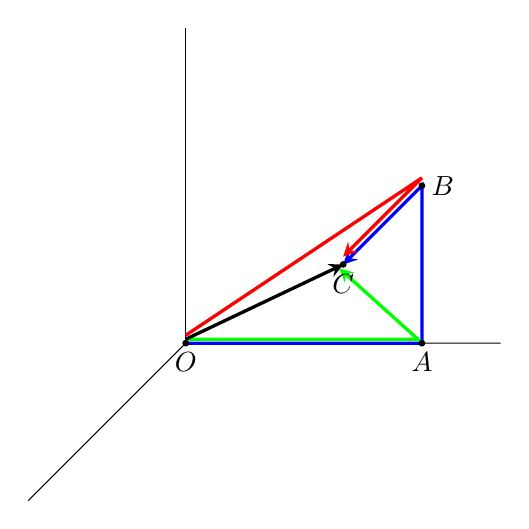
\begin{tikzpicture}
\draw (-2,-2) -- (0,0) -- (4,0);
\draw (0,0) -- (0,4);

\draw[-stealth, blue, very thick] (0,0) -- (3,0) -- (3,2) -- (2,1);


\draw[-stealth, green, very thick] (0,0+0.05) -- (3-0.05,0+0.05)-- (2-0.05,1-0.05);

\draw[-stealth, red, very thick] (0, 0 + 0.1) -- (3,2+0.1) -- (2,1+0.1);

\draw[-stealth, very thick] (0, 0.05) -- (2,1);
\filldraw[black] (0,0) circle (1pt) node[anchor=north]{$O$};
\filldraw[black] (3,0) circle (1pt) node[anchor=north]{$A$};
\filldraw[black] (3,2) circle (1pt) node[anchor=west]{$B$};
\filldraw[black] (2,1) circle (1pt) node[anchor=north]{$C$};

\end{tikzpicture}


Operator $T: C^{\infty}(S^1, \mathbb R^2) \to C^{\infty}(S^1, \mathbb R^2)$ by 
$T\xi = J(t)\frac{d}{dt}\xi + J(t)J_0 M\xi$, where 
$J(t)$ is a $t$-dependent complex structure on $\R^2$,
$J_0$ is the standard complex structure on $\R^2$,
$-J_0J(t) >0$ is positive definite,
$M$ is a constant symmetric matrix that does not have $0$ as an eigen-value. 
Can we find a inner product on $C^{\infty}(S^1, \mathbb R^2)$ such that $T$ is self-adjoint?


\end{document}
